\documentclass[11pt]{article}

\usepackage[margin=0.9in]{geometry}
\usepackage[T1]{fontenc}
\usepackage[utf8]{inputenc}
\usepackage{lmodern}
\usepackage{booktabs}
\usepackage{array}
\usepackage{siunitx}
\usepackage{amsmath}
\usepackage{tikz}
\usepackage{pgfplots}
\usepackage{subcaption}
\usepackage{xcolor}
\usepackage{hyperref}
\usepackage{enumitem}

\pgfplotsset{compat=1.18}
\sisetup{detect-all}

\definecolor{vcyan}{HTML}{00E5FF}
\definecolor{vgreen}{HTML}{76FF03}
\definecolor{vorange}{HTML}{FF9100}
\definecolor{vmagenta}{HTML}{D500F9}

\pgfplotsset{
  darkaxis/.style={
    width=\linewidth,
    height=5.5cm,
    axis background/.style={fill=black},
    grid=both,
    grid style={draw=gray!45},
    major grid style={draw=gray!55},
    axis line style={white},
    tick style={white},
    ticklabel style={color=white,font=\scriptsize},
    label style={color=white,font=\small},
    title style={color=white,font=\small\bfseries},
    legend style={draw=none, fill=black, text=white, font=\scriptsize},
    line join=bevel
  }
}

\title{\textbf{NeuroCore Workthrough:}\\
Transistor-Level Neuromorphic Compute to GDSII Flow Evidence}
\author{Project Log Date: 2026-02-02}
\date{}

\begin{document}
\maketitle

\begin{abstract}
This workthrough documents a reproducible hardware-development path built in one repository:
(1) analog neuromorphic circuits verified at transistor level in Spectre/OCEAN,
(2) a completed digital stack from CMOS primitives to GPU-core-level hierarchy, and
(3) a script-driven implementation smoke flow that reaches routed physical artifacts and GDSII output.
Unlike polished concept slides, the figures in this report are plotted directly from sampled electrical data points (no smoothing) with a dark-scope visual style for video-aligned evidence presentation.
\end{abstract}

\section{Project Snapshot}

\begin{table}[h]
\centering
\caption{Current execution status (competition-facing view).}
\begin{tabular}{>{\raggedright\arraybackslash}p{4.0cm} >{\raggedright\arraybackslash}p{2.0cm} >{\raggedright\arraybackslash}p{6.7cm}}
\toprule
\textbf{Track} & \textbf{Status} & \textbf{Evidence} \\
\midrule
Analog path (\texttt{synapse} \textrightarrow{} \texttt{neuro\_tile4\_coupled}) & PASS &
\texttt{competition/verification-evidence.md} \\
Digital hierarchy (CMOS \textrightarrow{} GPU core) & PASS &
\texttt{results/gpu\_core\_test.txt} \\
Robustness sweep (9-point matrix) & PASS (9/9) &
\texttt{competition/sweeps/neuro\_tile4\_coupled\_sweep\_summary.md} \\
Synopsys DC smoke & BLOCKED (license) &
\texttt{implementation/fullflow\_demo/work/dc/reports/alu4\_flow\_demo\_dc\_fallback.warn} \\
Cadence Innovus smoke & PASS &
\texttt{implementation/fullflow\_demo/work/innovus/out/alu4\_flow\_demo.gds} \\
Siemens Calibre smoke & BLOCKED (license) &
\texttt{implementation/fullflow\_demo/work/calibre/alu4\_flow\_demo\_drc.summary} \\
\bottomrule
\end{tabular}
\label{tab:status}
\end{table}

\begin{figure}[h]
\centering
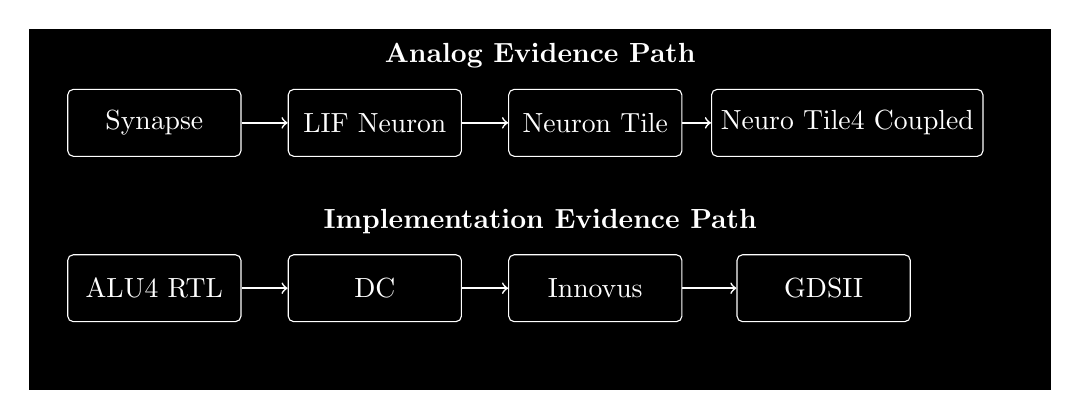
\begin{tikzpicture}[x=1cm,y=1cm]
  \fill[black] (0,0) rectangle (13,4.6);
  \draw[white, line width=0.5pt] (0,0) rectangle (13,4.6);

  \node[draw=white, rounded corners=2pt, fill=black, text=white, minimum width=2.2cm, minimum height=0.85cm] (a1) at (1.6,3.4) {Synapse};
  \node[draw=white, rounded corners=2pt, fill=black, text=white, minimum width=2.2cm, minimum height=0.85cm] (a2) at (4.4,3.4) {LIF Neuron};
  \node[draw=white, rounded corners=2pt, fill=black, text=white, minimum width=2.2cm, minimum height=0.85cm] (a3) at (7.2,3.4) {Neuron Tile};
  \node[draw=white, rounded corners=2pt, fill=black, text=white, minimum width=2.6cm, minimum height=0.85cm] (a4) at (10.4,3.4) {Neuro Tile4 Coupled};

  \node[draw=white, rounded corners=2pt, fill=black, text=white, minimum width=2.2cm, minimum height=0.85cm] (d1) at (1.6,1.3) {ALU4 RTL};
  \node[draw=white, rounded corners=2pt, fill=black, text=white, minimum width=2.2cm, minimum height=0.85cm] (d2) at (4.4,1.3) {DC};
  \node[draw=white, rounded corners=2pt, fill=black, text=white, minimum width=2.2cm, minimum height=0.85cm] (d3) at (7.2,1.3) {Innovus};
  \node[draw=white, rounded corners=2pt, fill=black, text=white, minimum width=2.2cm, minimum height=0.85cm] (d4) at (10.1,1.3) {GDSII};

  \draw[->,white,line width=0.6pt] (a1) -- (a2);
  \draw[->,white,line width=0.6pt] (a2) -- (a3);
  \draw[->,white,line width=0.6pt] (a3) -- (a4);
  \draw[->,white,line width=0.6pt] (d1) -- (d2);
  \draw[->,white,line width=0.6pt] (d2) -- (d3);
  \draw[->,white,line width=0.6pt] (d3) -- (d4);

  \node[text=white, font=\bfseries] at (6.5,4.25) {Analog Evidence Path};
  \node[text=white, font=\bfseries] at (6.5,2.15) {Implementation Evidence Path};
\end{tikzpicture}
\caption{End-to-end evidence structure used in the demo narrative.}
\label{fig:stack-diagram}
\end{figure}

\section{Raw Electrical Data (No Smoothing)}

\subsection{Synapse and Tile-Level Spiking}

\begin{figure}[h]
\centering
\begin{tikzpicture}
\begin{axis}[
  darkaxis,
  title={Synapse Waveforms (sampled points)},
  xlabel={Time (ns)},
  ylabel={Voltage (V)},
  xmin=0, xmax=120,
  ymin=0, ymax=1.8,
  legend pos=north east
]
  \addplot+[sharp plot, line width=0.35pt, mark=*, mark size=0.25pt, color=vcyan]
    table[x=time_ns,y=pre,col sep=comma]{../data/synapse_waveform.csv};
  \addplot+[sharp plot, line width=0.35pt, mark=*, mark size=0.25pt, color=vgreen]
    table[x=time_ns,y=post,col sep=comma]{../data/synapse_waveform.csv};
  \addplot+[sharp plot, line width=0.35pt, mark=*, mark size=0.25pt, color=vorange]
    table[x=time_ns,y=out,col sep=comma]{../data/synapse_waveform.csv};
  \legend{pre, post, out}
\end{axis}
\end{tikzpicture}
\caption{Synapse waveform traces plotted directly from sampled CSV points.}
\label{fig:synapse}
\end{figure}

\begin{figure}[h]
\centering
\begin{tikzpicture}
\begin{axis}[
  darkaxis,
  title={Neuro Tile4 Spike Channels (raw points)},
  xlabel={Time (ns)},
  ylabel={Spike Voltage (V)},
  xmin=0, xmax=120,
  ymin=0, ymax=0.85,
  legend pos=north west
]
  \addplot+[sharp plot, line width=0.35pt, mark=*, mark size=0.22pt, color=vcyan]
    table[x=time_ns,y=spike0,col sep=comma]{../data/neuro_tile4_spikes.csv};
  \addplot+[sharp plot, line width=0.35pt, mark=*, mark size=0.22pt, color=vgreen]
    table[x=time_ns,y=spike1,col sep=comma]{../data/neuro_tile4_spikes.csv};
  \addplot+[sharp plot, line width=0.35pt, mark=*, mark size=0.22pt, color=vorange]
    table[x=time_ns,y=spike2,col sep=comma]{../data/neuro_tile4_spikes.csv};
  \addplot+[sharp plot, line width=0.35pt, mark=*, mark size=0.22pt, color=vmagenta]
    table[x=time_ns,y=spike3,col sep=comma]{../data/neuro_tile4_spikes.csv};
  \legend{spike0, spike1, spike2, spike3}
\end{axis}
\end{tikzpicture}
\caption{Four-channel spiking behavior with measured first-spike staggering at 27.5/29.5/31.5/33.5 ns.}
\label{fig:tile4-spikes}
\end{figure}

\begin{figure}[h]
\centering
\begin{subfigure}[t]{0.49\linewidth}
\centering
\begin{tikzpicture}
\begin{axis}[
  darkaxis,
  title={Coupled Tile Spikes},
  xlabel={Time (ns)},
  ylabel={Voltage (V)},
  xmin=0, xmax=120,
  ymin=0, ymax=1.9,
  legend pos=north west
]
  \addplot+[sharp plot, line width=0.30pt, mark=*, mark size=0.20pt, color=vcyan]
    table[x=time_ns,y=spike0,col sep=comma]{../data/neuro_tile4_coupled_spikes.csv};
  \addplot+[sharp plot, line width=0.30pt, mark=*, mark size=0.20pt, color=vgreen]
    table[x=time_ns,y=spike1,col sep=comma]{../data/neuro_tile4_coupled_spikes.csv};
  \addplot+[sharp plot, line width=0.30pt, mark=*, mark size=0.20pt, color=vorange]
    table[x=time_ns,y=spike2,col sep=comma]{../data/neuro_tile4_coupled_spikes.csv};
  \addplot+[sharp plot, line width=0.30pt, mark=*, mark size=0.20pt, color=vmagenta]
    table[x=time_ns,y=spike3,col sep=comma]{../data/neuro_tile4_coupled_spikes.csv};
\end{axis}
\end{tikzpicture}
\end{subfigure}
\hfill
\begin{subfigure}[t]{0.49\linewidth}
\centering
\begin{tikzpicture}
\begin{axis}[
  darkaxis,
  title={Coupled Tile Membranes},
  xlabel={Time (ns)},
  ylabel={Voltage (V)},
  xmin=0, xmax=120,
  ymin=0, ymax=1.4,
  legend pos=north west
]
  \addplot+[sharp plot, line width=0.30pt, mark=*, mark size=0.20pt, color=vcyan]
    table[x=time_ns,y=mem0,col sep=comma]{../data/neuro_tile4_coupled_mems.csv};
  \addplot+[sharp plot, line width=0.30pt, mark=*, mark size=0.20pt, color=vgreen]
    table[x=time_ns,y=mem1,col sep=comma]{../data/neuro_tile4_coupled_mems.csv};
  \addplot+[sharp plot, line width=0.30pt, mark=*, mark size=0.20pt, color=vorange]
    table[x=time_ns,y=mem2,col sep=comma]{../data/neuro_tile4_coupled_mems.csv};
  \addplot+[sharp plot, line width=0.30pt, mark=*, mark size=0.20pt, color=vmagenta]
    table[x=time_ns,y=mem3,col sep=comma]{../data/neuro_tile4_coupled_mems.csv};
\end{axis}
\end{tikzpicture}
\end{subfigure}
\caption{Coupled-tile feed-forward propagation traces from sampled electrical data points.}
\label{fig:coupled-traces}
\end{figure}

\begin{table}[h]
\centering
\caption{Selected analog metrics extracted from verification artifacts.}
\begin{tabular}{lll}
\toprule
\textbf{Block} & \textbf{Metric} & \textbf{Value} \\
\midrule
Synapse & \(V_{\text{post,max}}\) & \SI{1.575}{V} \\
Synapse & Output pulse count & 6 \\
LIF neuron & Total spikes detected & 10 \\
LIF neuron & \(V_{\text{mem,max}}\) & \SI{1.573}{V} \\
Neuron tile & Spike-node pulses & 12 \\
Neuro Tile4 & First spike times & 27.5, 29.5, 31.5, 33.5 ns \\
Neuro Tile4 Coupled & Membrane maxima & 0.569, 0.974, 1.268, 0.873 V \\
Neuro Tile4 Coupled & Spike counts & 15, 15, 1, 1 \\
\bottomrule
\end{tabular}
\label{tab:analog-metrics}
\end{table}

\section{Robustness Sweep Evidence}

\begin{figure}[h]
\centering
\begin{tikzpicture}
\begin{axis}[
  darkaxis,
  title={Sweep: Membrane Channel-2 Peak vs \(r_{fb}\)},
  xlabel={\(r_{fb}\) (Ohm)},
  ylabel={\(V_{\text{mem2,max}}\) (V)},
  xmin=650, xmax=1550,
  ymin=1.20, ymax=1.31,
  legend pos=south west
]
  \addplot+[sharp plot, mark=*, mark size=1.4pt, line width=0.6pt, color=vcyan]
    table[x=r_fb_ohm,y=mem2_max_v,col sep=comma]{data/sweep_mem2_rleak_6000000.csv};
  \addplot+[sharp plot, mark=square*, mark size=1.3pt, line width=0.6pt, color=vgreen]
    table[x=r_fb_ohm,y=mem2_max_v,col sep=comma]{data/sweep_mem2_rleak_8000000.csv};
  \addplot+[sharp plot, mark=triangle*, mark size=1.4pt, line width=0.6pt, color=vorange]
    table[x=r_fb_ohm,y=mem2_max_v,col sep=comma]{data/sweep_mem2_rleak_10000000.csv};
  \legend{\(r_{leak}=6\,\text{M}\Omega\), \(r_{leak}=8\,\text{M}\Omega\), \(r_{leak}=10\,\text{M}\Omega\)}
\end{axis}
\end{tikzpicture}
\caption{9-point robustness sweep plotted from parsed sweep CSV (\texttt{PASS}=9/9).}
\label{fig:sweep}
\end{figure}

\begin{table}[h]
\centering
\caption{Sweep envelope summary from \texttt{neuro\_tile4\_coupled\_sweep\_parsed.csv}.}
\begin{tabular}{lcc}
\toprule
\textbf{Metric} & \textbf{Minimum} & \textbf{Maximum} \\
\midrule
\(V_{\text{mem0,max}}\) & 0.561 V & 0.575 V \\
\(V_{\text{mem1,max}}\) & 0.957 V & 0.984 V \\
\(V_{\text{mem2,max}}\) & 1.226 V & 1.293 V \\
\(V_{\text{mem3,max}}\) & 0.869 V & 0.876 V \\
Spike-count vector \((s0,s1,s2,s3)\) & \multicolumn{2}{c}{(15, 15, 1, 1) at all 9 points} \\
\bottomrule
\end{tabular}
\label{tab:sweep-envelope}
\end{table}

\section{Implementation Flow Artifacts}

\begin{table}[h]
\centering
\caption{Full-flow smoke outputs for \texttt{alu4\_flow\_demo}.}
\begin{tabular}{>{\raggedright\arraybackslash}p{2.2cm} >{\raggedright\arraybackslash}p{1.8cm} >{\raggedright\arraybackslash}p{7.0cm}}
\toprule
\textbf{Stage} & \textbf{Result} & \textbf{Artifact(s)} \\
\midrule
DC & Blocked (license) & \texttt{dc\_shell.log}, fallback mapped netlist \\
Innovus & PASS & \texttt{alu4\_flow\_demo.def}, \texttt{alu4\_flow\_demo.gds}, post-route netlist \\
Calibre DRC & Blocked (license) & \texttt{alu4\_flow\_demo\_drc.summary} \\
\midrule
Area (Innovus) & --- & 10 instances, total area = 20.520 \\
Power (Innovus) & --- & total power = 0.00069651 mW \\
\bottomrule
\end{tabular}
\label{tab:fullflow}
\end{table}

\section{Reproducibility Commands}

\begin{itemize}[leftmargin=1.2em]
  \item Build and verify stack: \texttt{source setup\_cadence.sh} then \texttt{./build.sh all}
  \item Refresh competition visuals: \texttt{scripts/run\_competition\_visuals.sh}
  \item Parse paper helper data: \texttt{python3 scripts/prepare\_paper\_data.py}
  \item Full-flow smoke replay: \texttt{scripts/run\_fullflow\_smoke.sh}
  \item Strict mode (fail on blocked stages): \texttt{FULLFLOW\_STRICT=1 scripts/run\_fullflow\_smoke.sh}
\end{itemize}

\section{Conclusion}

This repository now demonstrates a practical and auditable path from transistor-level
analog neuromorphic behavior to physical implementation artifacts.
The key contribution for competition use is not a single benchmark number but a
repeatable engineering chain:
\textit{measured electrical traces, robustness sweeps, scripted implementation flow,
and concrete GDSII output artifacts}.
That combination is designed to be shown live in one terminal session and defended
with raw-source files.

\end{document}
